\section{Zielsetzung}
In diesem Versuch zur Rutherfordstreuung soll die Wechselwirkung von $\alpha$-Teilchen mit einer Goldfolie untersucht werden.
Im weiteren Verlauf werden weitere Materialien wie Bismut und Aluminium untersucht.

\section{Historisches}
Bevor Rutherford seinen bekannten Streuversuch durchführte war das Thomson'sche Atommodell das verbreitetste Modell. In diesem,
auch als Rosinenkuchen-Modell bekannten Atommodell, wird von einer homogen verteilten positiven Ladung ausgegangen, in der die
negativ geladenen Elektronen wie Rosinen verteilt sind. Rutherford zeigte durch seinen Streuversuch, dass das Atom aus einem
Kern aufgebaut ist, in dem nahezu die ganze Masse konzentriert ist und von Elektronen umkreist wird.

\section{Theorie}
Für diesen Versuch wird $\alpha$-Strahlung verwendet. Diese besteht aus einem zweifach positiv geladenem Heliumkern, also
zwei Protonen und zwei Neutronen. Durchquert  diese Strahlung Materie kann sie mit dieser auf verschiedene Weisen wechselwirken.
Bei der Wechselwirkung mit den Hüllenelektronen der durchstrahlten Materie kommt es aufgrund der großen Massendifferenz der
$\alpha$-Teilchen und der Hüllenelektronen nur zu einem geringen Impulsübertrag auf das $\alpha$-Teilchen und somit nur zu einer
minimalen Richtungsänderung. Der Energieverlust des $\alpha$-Teichens bzw. der Energieübertrag auf das Hüllenelektron ist
hingegen nicht zu vernachlässigen. Dieser Energieverlust pro Weglängeneinheit wird durch die Bethe-Bloch Formel

\begin{equation}
  -\frac{dE}{dx}=\frac{4\pi e^4 z²NZ}{m_0 v^2 (4\pi \epsilon_0)^2}\cdot\ln\Bigg(\frac{2m_0 v²}{I}\Bigg)
  \label{eqn:BetheBloch}
\end{equation}

beschrieben.
Dabei ist $z$ die Ladung des $\alpha$-Teilchens, $Z$ die Kernladungszahl der durchstrahlten Materie, N die Anzahl der
Teilchen pro $\si{\cm\squared}$, $m_0$ die Ruhemasse des Elektrons, $v$ dessen Geschwindigkeit und $I$ die mittlere
Ionisationsenergie.

Des Weitern können die $\alpha$-Teilchen auch aufgrund der Coulobkraft am Atomkern gestreut werden, wodurch sie eine
Richtungsänderung erfahren. Daraus leitete Rutherford die Rutherford'sche Streuformel
\begin{equation}
  \frac{d\sigma}{d\Omega}(\Phi)=\frac{1}{(4\pi \epsilon_0)^2}\Bigg(\frac{zZe^2}{4E_{\alpha}}\Bigg)^2
  \cdot\frac{1}{\sin^4{(\frac{\Phi}{2})}}
  \label{eqn:Rutherford}
\end{equation}

her, welche den differentiellen Wirkungsquerschnitt in Abhängigkeit des Streuwinkels $\Phi$ angibt. Mit $E_{\alpha}$
wird hier die kinetische Energie des $\alpha$-Teilchens bezeichnet.

\subsection{Americium}

Als radioaktive Quelle wird $\ce{^{241} Am}$ verwendet. Dies ist ein silbrig-weißes Metall mit einer
Halbwertszeit von 433 Jahren. Primär geht von dieser Quelle $\alpha$-Strahlung mit einer Energie von
$E_{\alpha}=\SI{5,48}{\eV}$ aus. Beim Übergang des angeregten Kerns in den Grundzustand werden auch geringe
Mengen an $\gamma$-Strahlung emittiert. Diese Prozesse sind im Zerfallsschema in Abbildung \ref{fig:Zerfall}
dargestellt.

\begin{figure}[H]
  \centering
  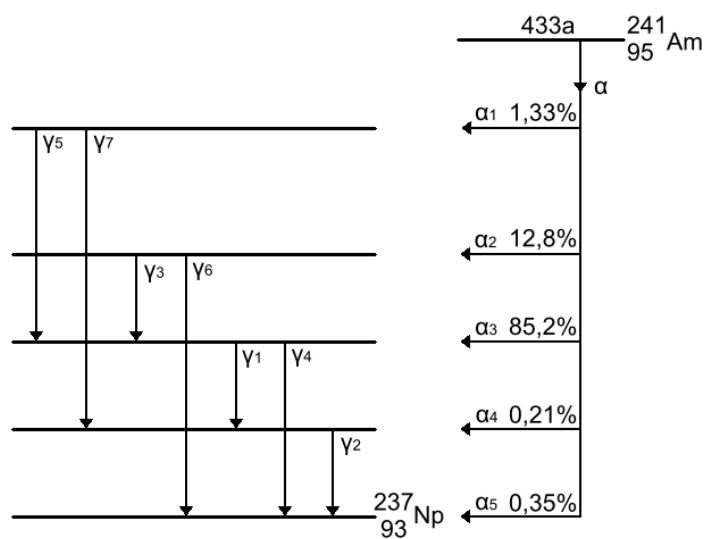
\includegraphics[width=8cm]{Zerfallsschema.png}
  \caption{Zerfallsschema von $\ce{^{241} Am}$. }
  \label{fig:Zerfall}
  \cite{zerfall}
\end{figure}

\subsection{Surface-Barrier Detektor}
Um die gestreute $\alpha$-Strahlung zu detektieren wird ein Surface-Barrier Detektor
(dt. Oberflächensperrschichtzähler) verwendet, welcher zu den Halbleiterdetektoren zählt.
Ein schematische Aufbau dieses Detektors ist in Abbildung \ref{fig:detektor} dargestellt.
Dieser besteht aus Silizium als Ausgangsmaterial, welches durch verschiedene Materialien
p- und n-dotiert wird. Zwischen dieser p- und n- dotierten Schicht bildet sich eine Verarmungszone,
welche den eigentlichen Detektorbereich bildet. Durch anlegen einer äußeren Spannung kann diese
Verarmungszone vergrößert werden.

Das besondere an einem Surface-Barrier Detektor ist, wie der Name schon
sagt, die besondere Oberflächenempfindlichkeit, da die Verarmungszone sehr nah an der Oberfläche liegt.
Dies ist für die Detektion von $\alpha$-Teilchen auch notwendig, da diese nach der Bethe-Bloch Formel
pro Wegstrecke sehr viel Energie verlieren.

\begin{figure}[H]
  \centering
  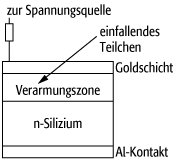
\includegraphics[width=5cm]{detektor.png}
  \caption{Aufbau eines Surface-Barrier Detektors.}
  \label{fig:detektor}
  \cite{detektor}
\end{figure}

\subsection{Drehschieberpumpe}
Um die Vakuumkammer zu evakuieren wird in diesem Versuch eine Drehschieberpumpe verwendet, welche
einen Vakuum mit ca. $\SI{70}{\milli\bar}$ erzeugt. Der prinzipielle Aufbau einer solchen Pumpe ist in
Abbildung \ref{fig:Drehschieber} dargestellt. Die Schieber befinden sich auf einem Rotor und werden
durch Federn an die Rotorwand gedrückt. Dieser Übergang muss dicht sein, damit duch Rotation ein
Vakuum entsteht, welches die Luft aus dem Einlass ansaugt. Diese Luft wird dann durch die Schieber
bis zum Auslassventil bewegt und an die Atmosphäre abgegeben.

\begin{figure}[H]
  \centering
  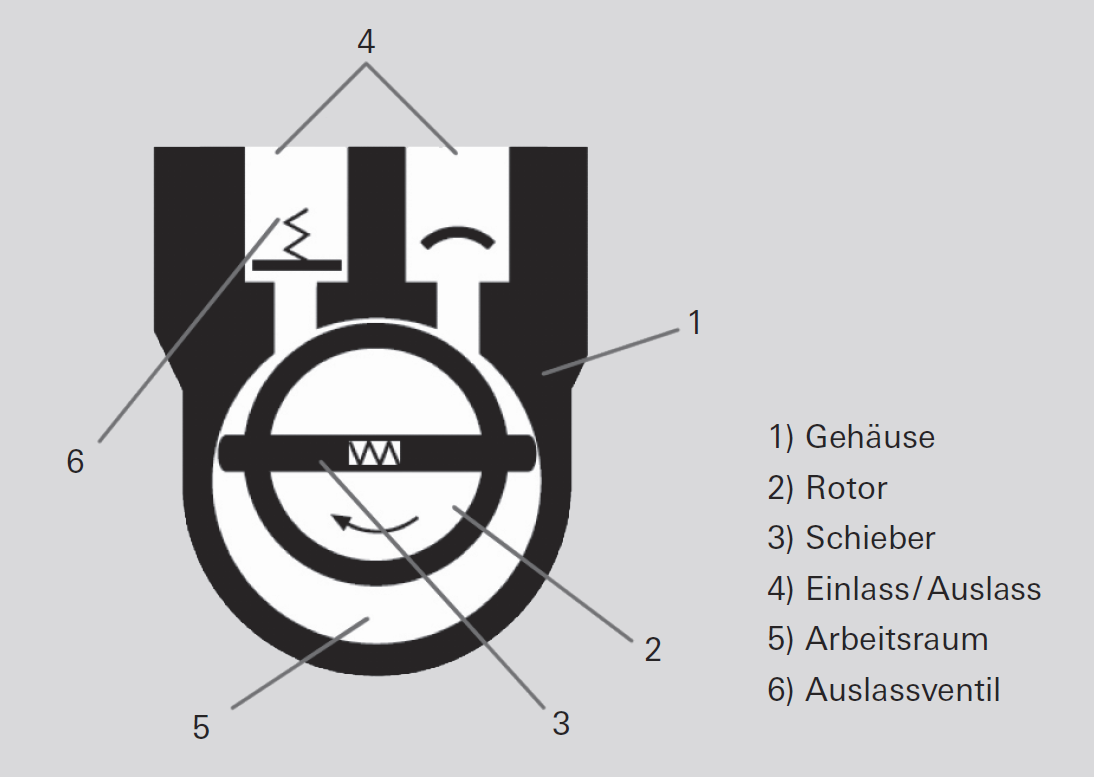
\includegraphics[width=8cm]{Drehschieber.png}
  \caption{Schematischer Aufbau einer Drehschieberpumpe.}
  \label{fig:Drehschieber}
\end{figure}
